
\documentclass{report}

\input{preamble}
\input{macros}
\input{letterfonts}

\title{\Huge{Programmazione Cross-Platform con Flutter}\\Sistemi Informativi Aziendali}
\author{\huge{Caberlotto Giovanni}}
\date{}

\begin{document}

\maketitle
\newpage% or \cleardoublepage
% \pdfbookmark[<level>]{<title>}{<dest>}
\pdfbookmark[section]{\contentsname}{toc}
\tableofcontents
\pagebreak

\chapter{Introduzione al linguaggio dart} % (fold)
\label{chap:Introduzione al linguaggio dart}
\\
\section{Perché Dart}
\\
Dart è un linguaggio di programmazione moderno, di alto livello e di uso generale sviluppato originariamente da Google. Benché sia emerso nel 2011, la sua versione stabile è stata rilasciata nel giugno 2017. Sebbene inizialmente non fosse molto popolare, ha guadagnato notorietà grazie all'utilizzo nel framework Flutter
\\
\\
Dart è un linguaggio di programmazione dinamico, basato su classi e orientato agli oggetti, incorporando concetti come chiusure e ambito lessicale. La sua sintassi è notevolmente simile a linguaggi come Java, C, e JavaScript, facilitando il processo di apprendimento per chi è già familiare con uno di questi linguaggi.
\\
L'ampio utilizzo di Dart è evidente nello sviluppo di una vasta gamma di applicazioni, inclusi:
\begin{itemize}
  \item{Applicazioni Mobili: Dart è diventato noto principalmente grazie al suo utilizzo nel framework Flutter, ampiamente adottato per lo sviluppo di app mobili multi-piattaforma}
  \item{Applicazioni Web Moderne: Dart è utilizzato per la creazione di applicazioni web moderne, fornendo una solida base per lo sviluppo di frontend e backend}
  \item{Applicazioni Desktop: Dart può essere utilizzato anche per lo sviluppo di applicazioni desktop, offrendo versatilità nelle applicazioni software}
  \item{Internet of Things (IoT): La sua flessibilità lo rende adatto anche per lo sviluppo di applicazioni IoT}
\end{itemize}
\\
Dart supporta una serie di concetti avanzati, tra cui:
\\
\begin{itemize}
  \item{Interfacce: Consentono la definizione di contratti di implementazione, fornendo una struttura per la progettazione di codice modulare}
  \item{Mixin: Permettono la composizione di comportamenti in classi, migliorando la riusabilità del codice}
  \item{Classi Astratte: Forniscono una base per la creazione di gerarchie di classi, permettendo l'implementazione di metodi comuni}
  \item{Generics: Consentono la creazione di codice più flessibile e riutilizzabile attraverso la parametrizzazione di tipi}
  \item{Reified Generics: Offrono supporto per la manipolazione dei tipi a tempo di esecuzione}
\end{itemize}
\\
Dart è un linguaggio compilato e supporta due principali tecniche di compilazione:
\\
\begin{itemize}
  \item{AOT (Ahead of Time): Converte il codice Dart in codice JavaScript ottimizzato tramite il compilatore dar2js. Questo processo avviene in fase di compilazione e consente l'esecuzione su tutti i moderni browser web}
  \item{JIT (Just-In-Time): Converte il codice Dart bytecode direttamente in codice nativo, ottimizzando solo il codice effettivamente necessario durante l'esecuzione.}
\end{itemize}
\\
Dart, grazie alla sua sintassi familiare, versatilità e integrazione con Flutter, è diventato un linguaggio di programmazione sempre più adottato. Con il supporto per concetti avanzati e le tecniche di compilazione AOT e JIT, Dart si posiziona come una scelta solida per lo sviluppo di una vasta gamma di applicazioni moderne.
\\
\\
Dart è stato presentato per la prima volta alla conferenza GOTO, tenutasi dal 10 al 12 ottobre 2011 ad Aarhus, Danimarca. Inizialmente progettato da Lars Bak e Kasper Lund, Dart è stato sviluppato da Google
\\
\\
La prima versione stabile di Dart, la 1.0, è stata rilasciata il 14 novembre 2013, con l'ambizione di essere considerata una possibile sostituzione per JavaScript. Tuttavia, questa mossa ha ricevuto critiche, soprattutto per le sfide nell'adozione sul web
\\
\\
Nel luglio 2014, la prima edizione del linguaggio Dart è stata ufficialmente approvata da Ecma International durante la sua 107a Assemblea Generale. Ciò ha indicato un passo importante verso la standardizzazione del linguaggio
\\
\\
Nonostante gli sforzi iniziali, la prima versione di Dart ha incontrato ostacoli e è stata criticata per alcune problematiche, specialmente riguardo all'adozione sul web. Questo ha portato all'abbandono del progetto nel 2015, con la release 1.9 di Dart. Tuttavia, questo non ha segnato la fine della storia di dart
\\
\\
Dart ha vissuto una rinascita con il rilascio della sua seconda versione, Dart 2.0, nel mese di agosto. Uno dei cambiamenti significativi è stato l'introduzione di un sistema di tipi sonori, mirato a migliorare la sicurezza del tipo durante la compilazione e l'esecuzione del codice. Questa nuova versione ha portato ad una maggiore adozione e interesse nella comunità di sviluppatori
\\
\\
La recente versione di Dart, la 2.7, ha introdotto il concetto di "metodo delle estensioni". Questa caratteristica consente agli sviluppatori di aggiungere nuove funzionalità a qualsiasi tipo di dati senza modificarne il codice sorgente originale. Questa capacità di estendere le funzionalità dei tipi ha ampliato ulteriormente le possibilità di sviluppo in Dart
\\
\\
Dart ha attraversato una serie di fasi nella sua evoluzione, inizialmente affrontando sfide e critiche, ma successivamente trovando nuova vitalità con miglioramenti significativi nelle versioni successive. L'introduzione del sistema di tipi sonori e del metodo delle estensioni ha contribuito a consolidare la posizione di Dart come un linguaggio di programmazione moderno e versatile, specialmente nel contesto dello sviluppo di applicazioni con Flutter
\\
\\
Caratteristiche del linguaggio:
\\
\begin{itemize}
  \item{Indipendenza dalla Piattaforma:
Dart è un linguaggio indipendente dalla piattaforma, il che significa che può essere utilizzato su una varietà di sistemi operativi, inclusi Windows, Mac, Linux e altri. Ciò favorisce la portabilità delle applicazioni sviluppate in Dart}
  \item{Open Source:
Dart è un linguaggio open-source, il che significa che il suo codice sorgente è disponibile gratuitamente per tutti. Dotato di una licenza BSD, offre la libertà di utilizzarlo, modificarlo e distribuirlo senza restrizioni. Inoltre, il riconoscimento da parte dello standard ECMA contribuisce alla sua legittimità e standardizzazione}
  \item{Orientato agli Oggetti:
Dart è un linguaggio di programmazione orientato agli oggetti (OOP) e supporta tutte le caratteristiche fondamentali dell'OOP, come l'ereditarietà, le interfacce e i tipi opzionali. Questa progettazione orientata agli oggetti favorisce la modularità e la manutenibilità del codice}
  \item{Utilità per Applicazioni in Tempo Reale:
Grazie alla sua stabilità e alle caratteristiche di programmazione concorrente, Dart è particolarmente utile per lo sviluppo di applicazioni in tempo reale. La gestione efficiente degli eventi e la sintassi chiara contribuiscono a creare applicazioni reattive e performanti}
  \item{Compilatore dar2js:
Dart è dotato del compilatore dar2js, che traduce il codice Dart in codice JavaScript ottimizzato. Questa conversione consente all'applicazione Dart di essere eseguita su tutti i moderni browser web, consentendo una più ampia distribuzione delle applicazioni sviluppate con Dart}
  \item{VM Dart Stand-alone:
Dart include una Virtual Machine (VM) stand-alone che consente l'esecuzione del codice Dart in un ambiente con interfaccia a riga di comando (CLI). Questa funzionalità è utile per l'esecuzione di script Dart senza la necessità di un browser, fornendo flessibilità nell'utilizzo del linguaggio}
\end{itemize}
\\
Le caratteristiche di Dart, tra cui la sua indipendenza dalla piattaforma, lo status open-source, la natura orientata agli oggetti, la sua utilità per applicazioni in tempo reale e le opzioni di compilazione, lo rendono un linguaggio versatile e adatto a una gamma diversificata di progetti di sviluppo software
\\
\\
Concetti chiave del linguaggio Dart
\\
\begin{itemize}
  \item{Ogni cosa è un Oggetto:
In Dart, ogni entità è trattata come un oggetto, che include numeri, booleani, funzioni e altro. Questo concetto è simile a Python, dove tutto è un oggetto. Inoltre, tutti gli oggetti ereditano dalla classe Object, fornendo una base comune per la programmazione orientata agli oggetti}
  \item{Segnalazione di Problemi:
Gli strumenti di Dart possono segnalare due tipi di problemi durante la codifica: 
\begin{itemize}
  \item{Avvertimenti: Indicano che il codice potrebbe avere qualche problema, ma non impediscono l'esecuzione del codice. Possono servire come suggerimenti per migliorare la qualità del codice}
  \item{Errori: Possono impedire l'esecuzione del codice. Gli errori devono essere corretti prima che il programma possa essere eseguito con successo}
\end{itemize}
}
  \item{Digitazione dei Suoni:
Dart supporta la "digitazione dei suoni" (sound typing), un concetto che verrà approfondito in tutorial successivi. In breve, questo significa che il sistema di tipo di Dart può rilevare e prevenire alcuni errori di tipo durante la fase di compilazione, migliorando la sicurezza e la stabilità del codice}
  \item{Tipi Generici:
Dart supporta l'utilizzo di tipi generici, consentendo la dichiarazione di tipi specifici per le collezioni, come List<int> per un elenco di interi o List<dynamic> per un elenco di oggetti di qualsiasi tipo. Questa caratteristica aumenta la flessibilità del linguaggio e aiuta a scrivere codice più robusto}
\end{itemize}
\\
\section{Sintassi base}
\\
\subsubsection{Primo programma}
\\
Il metodo migliore per comprendere un linguaggio di programmazione è la metodologia learn by doing, seguendo questa filosofia, scriviamo ed eseguiamo il programma seguente:
\\
\\
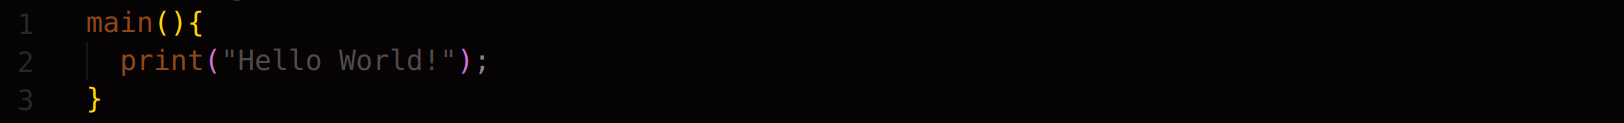
\includegraphics[width=0.8\textwidth]{./graphs/firstDartProgram.png}
\\
\\
La funzione main() indica che è l'inizio del nostro programma. È una funzione essenziale in cui il programma inizia la sua esecuzione
\\
\\
La funzione print() viene utilizzata per visualizzare l'output sulla console. È simile a quella del C, di JavaScript o di qualsiasi altro linguaggio. Le parentesi graffe e i punti e virgola sono necessari per un uso appropriato.
\\
\\
Per compilare ed eseguire il programma basta aprire il terminale e digitare il seguente comando, dove helloworld.dart rappresenta il file
\\
\\
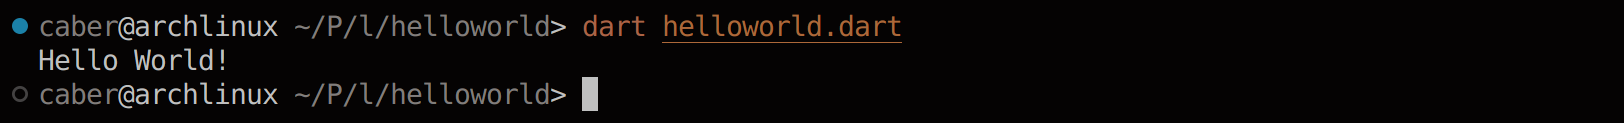
\includegraphics[width=0.8\textwidth]{./graphs/compilazioneProgrammaDart.png}
\\
\subsubsection{Identificatori}
\\
Gli identificatori sono i nomi utilizzati per definire variabili, metodi, classi e funzioni, ecc. Un identificatore è una sequenza di lettere([dalla A alla Z],[dalla a alla z]), cifre([0-9]) e trattini bassi(\_), il primo carattere non deve essere numerico. Esistono alcune regole per definire gli identificatori, riportate di seguito.
\\
\begin{itemize}
  \item{Il primo carattere non deve essere una cifra}
  \item{Non sono ammessi caratteri speciali, tranne il trattino basso (\_) o il segno del dollaro (\$)}
  \item{Non sono ammessi due trattini bassi consecutivi (\_\_)}
  \item{Il primo carattere deve essere un alfabeto (maiuscolo o minuscolo) o un trattino basso}
  \item{Gli identificatori devono essere unici e non possono contenere spazi}
  \item{Sono case sensitive le variabili Y e y non vengono trattate alla stessa maniera}
\end{itemize}
\\
\subsubsection{Stampa e interpolazione di stringhe}
\\
La funzione print() è usata per stampare l'output sulla console e \$\{expression\} è usata per l'interpolazione delle stringhe. Di seguito è riportato un esempio.
\\
\\
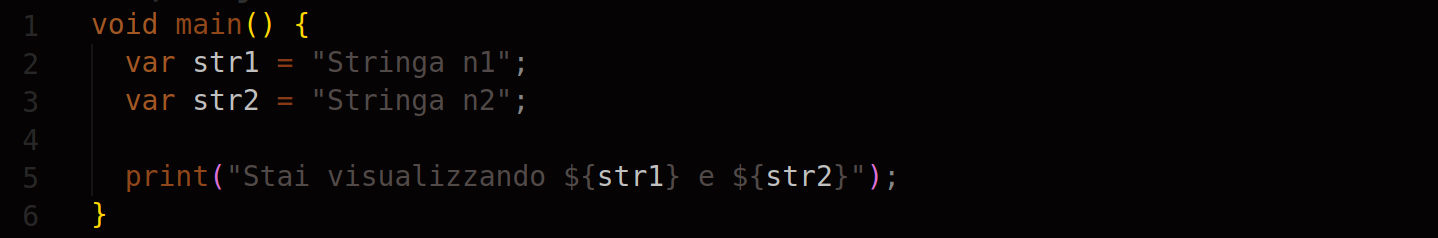
\includegraphics[width=0.8\textwidth]{./graphs/StrPrintingeInterpolazione.png}
\\
\textbf{output}
\\
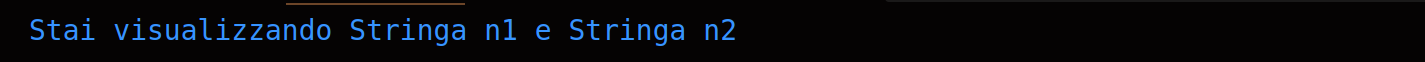
\includegraphics[width=0.8\textwidth]{./graphs/outputPrintingStreInterpolazione.png}
\subsubsection{Punto e virgola}
\\
Il punto e virgola viene utilizzato per terminare l'istruzione, cioè per indicare che l'istruzione termina qui. È obbligatorio che ogni istruzione sia terminata con un punto e virgola(;). È possibile scrivere più istruzioni in una singola riga utilizzando il punto e virgola come delimitatore. Il compilatore genera un errore se non viene utilizzato correttamente.
\\
\subsubsection{Spazi e interruzione di riga}
\\

% chapter Introduzione al linguaggio dart (end)

\chapter{Flutter} % (fold)
\label{chap:Flutter}

% chapter Flutter (end)

\end{document}
